\documentclass[a4paper,11pt]{article}

\usepackage[a4paper, margin=2.5cm]{geometry}
\usepackage[utf8]{inputenc}
\usepackage[T1]{fontenc}
\usepackage{mathptmx}
\usepackage{amsmath,amssymb}
\usepackage{graphicx}
\usepackage{booktabs}
\usepackage{longtable}
\usepackage{array}
\usepackage{tabularx}
\usepackage{caption}
\usepackage{subcaption}
\usepackage{hyperref}
\usepackage{xcolor}
\usepackage{fancyhdr}

\hypersetup{
  colorlinks=true,
  linkcolor=blue!60!black,
  citecolor=blue!60!black,
  urlcolor=blue!60!black
}

\renewcommand{\thesection}{S\arabic{section}}
\renewcommand{\thesubsection}{S\arabic{section}.\arabic{subsection}}
\renewcommand{\thefigure}{S\arabic{figure}}
\renewcommand{\thetable}{S\arabic{table}}

\pagestyle{fancy}
\fancyhf{}
\fancyhead[L]{\textit{Five Axes of Fragility} --- Supplementary Information}
\fancyhead[R]{\thepage}
\renewcommand{\headrulewidth}{0.4pt}

\title{\textbf{Supplementary Information}\\[6pt]
\large Five Axes of Fragility: A Systematic Robustness Audit of\\
Gene-Regulatory-Network Inference from Single-Cell Foundation Models}
\author{Ihor Kendiukhov}
\date{}

\begin{document}
\maketitle
\thispagestyle{fancy}

\tableofcontents
\listoffigures
\listoftables

\vspace{1em}
\noindent\hrulefill

\noindent
This supplement accompanies the main manuscript. It contains:
the panel registry and preprocessing parameters
(Supplementary Methods~S1, Table~S1); the adversarial AI-assisted
review protocol with the 27-issue full-census audit
(Supplementary Methods~S2); the Axis-3 per-cell-type reliability
metrics (Table~S3); and the seven supplementary figures referenced
from the main text (Figures~S1--S7). All section, table, and figure
references in the main paper resolve to items in this document.

% =====================================================================
% SUPPLEMENTARY METHODS S1
% =====================================================================
\clearpage
\section{Panel registry and preprocessing parameters}
\label{sec:supp_methods_s1}

This section freezes the TF--target panel definitions and preprocessing
choices that underpin every numerical result in the main paper. A
reviewer may treat it as ground truth for any claim the Methods
section makes about panel construction, normalization, HVG selection,
or gene filtering.

\subsection{Panel registry}

Every axis loads its TF--target panel from a single registry
(\texttt{fragility.panels.registry}) so cross-axis comparisons are
anchored to documented panels rather than ad-hoc gene lists.
Table~\ref{tab:s1} summarises the named panels and reproduces the full
gene lists for the \texttt{hematopoiesis\_76x108} panel used in Axis~4
(donor generalisation) and \S3.6 (scorer divergence).

\subsubsection*{Selection criteria for \texttt{hematopoiesis\_76x108}}

This panel is a deliberately dense Cartesian product because Axis~4
measures \emph{transfer} between donor splits, not literature
precision. Selection criteria (in response to R1b\,$\cdot$\,iii):

\begin{enumerate}
\item Start from the 76 hematopoiesis / immune TFs curated from
  DoRothEA confidence tiers A--C (Garcia-Alonso et al., 2019) and
  TRRUST (Han et al., 2018).
\item Intersect target candidates with a 108-gene immune /
  cross-tissue marker pool covering lineage markers, cytokines,
  surface molecules, costimulatory / checkpoint molecules, ECM
  components, lung epithelial markers, and housekeeping controls.
\item Emit the full Cartesian product $76 \times 108 = 8{,}208$
  directed edges. After dataset-specific gene-universe restriction
  (e.g.\ to kidney), 75 of 76 TFs and 99 of 108 targets remain,
  yielding 7{,}425 directed edges (the value used in \S3.6).
\end{enumerate}

\begin{table}[ht]
\centering
\caption{Named TF--target panels and the full gene lists for the
\texttt{hematopoiesis\_76x108} panel. Edge counts are reported
\emph{before} dataset-specific gene-universe restriction; restriction
reduces edge count by 10--40\% depending on the cohort.}
\label{tab:s1}
\small

\textbf{(A) Named panels in the registry}

\begin{tabularx}{\textwidth}{l X r l}
\toprule
\textbf{Panel name} & \textbf{Description} & \textbf{Edges} & \textbf{Used in} \\
\midrule
\texttt{primary} &
  DoRothEA confidence A/B (Garcia-Alonso et al., 2019)\,$\cap$\,TRRUST
  (Han et al., 2018) &
  3{,}384 & Axis~3 (shared-panel run) \\
\addlinespace
\texttt{dorothea\_ab} &
  DoRothEA confidence tiers A and B (Garcia-Alonso et al., 2019) &
  $\sim$11{,}000 & Axis~5 reference precision \\
\addlinespace
\texttt{trrust} &
  TRRUST v2 manually curated TF--target interactions (Han et al., 2018) &
  $\sim$8{,}500 & Axis~5 reference precision \\
\addlinespace
\texttt{hematopoiesis\_76x108} &
  76 hematopoiesis / immune TFs $\times$ 108 cross-tissue immune /
  marker targets (Cartesian product, see panel B below) &
  8{,}208 & Axis~4, scorer-divergence (\S3.6) \\
\addlinespace
\texttt{shared\_36} &
  TRRUST-intersected activation/repression panel for cross-dataset
  Axis~3 sensitivity &
  36 & Axis~3 sensitivity check \\
\bottomrule
\end{tabularx}

\vspace{1em}
\textbf{(B) Full gene lists for \texttt{hematopoiesis\_76x108}}

\begin{tabularx}{\textwidth}{l X}
\toprule
\textbf{76 TFs} &
STAT1, STAT3, STAT4, STAT5A, STAT5B, STAT6,
IRF1, IRF4, IRF7, IRF8,
NFKB1, NFKB2, RELA, REL, RELB,
TBX21, GATA3, RORC, FOXP3, BCL6,
SPI1, RUNX1, RUNX3, ETS1, ETS2,
MYC, MAX, JUN, FOS, JUNB, JUND, FOSL1, FOSL2,
HIF1A, EPAS1, ARNT,
TP53, RB1, E2F1, E2F4,
PAX5, EBF1, TCF7, LEF1,
CEBPA, CEBPB, CEBPD,
SOX2, SOX4, SOX9,
KLF2, KLF4, KLF6,
NR4A1, NR4A2, NR4A3,
BATF, BATF3, MAF, MAFB,
EOMES, PRDM1, ID2, ID3,
NFE2L2, BACH1, BACH2,
ZEB1, ZEB2, SNAI1, TWIST1,
FOXO1, FOXO3, AHR,
IKZF1, IKZF3 \\
\midrule
\textbf{108 targets} &
CD3D, CD3E, CD4, CD8A, CD8B, CD19, MS4A1, CD79A, CD79B,
CD14, CD68, ITGAM, ITGAX, FCGR3A, CSF1R,
IL2, IL2RA, IL7R, IL6, IL10, IL17A, IL21, IL4, IL13,
IFNG, TNF, TNFRSF9, TNFRSF18,
GZMB, GZMA, GZMK, PRF1, GNLY, NKG7,
CCL5, CCR7, CXCR4, CXCL13, CCL2, CXCL10,
HLA-DRA, HLA-DRB1, HLA-A, HLA-B, HLA-C, B2M,
LYZ, S100A8, S100A9, S100A12,
SELL, ITGA4, ITGB1, ICAM1, VCAM1,
MKI67, TOP2A, CDK1, PCNA,
BCL2, BCL2L1, MCL1, BAX, BAK1,
CTLA4, PDCD1, LAG3, HAVCR2, TIGIT, TOX,
FN1, COL1A1, COL3A1, VIM, ACTA2,
CDH1, EPCAM, SFTPC, SFTPB, SFTPA1, SCGB1A1, MUC5AC, FOXJ1,
PECAM1, CDH5, VWF, KDR, NOTCH1, DLL4, JAG1,
WNT5A, CTNNB1,
TGFB1, TGFBR1, SMAD3, SMAD7,
SOD2, HMOX1, NQO1, GSTP1,
GAPDH, ACTB, RPL13A, RPS18,
PTPRC, THY1, ENG, NT5E \\
\bottomrule
\end{tabularx}
\end{table}

\subsection{Preprocessing parameters}

The canonical pipeline is depth-normalize ($\texttt{target\_sum} = 10{,}000$
via \texttt{scanpy.normalize\_total}) followed by \texttt{log1p}
transformation, with the top 600 highly-variable genes selected via the
\texttt{seurat\_v3} flavour (Stuart et al., 2019). Gene filtering is at
$\geq 10$ cells per gene at load time. Every figure in \S3.1--\S3.5 of
the main paper is computed under these defaults.

The default HVG count of 600 was chosen for direct comparability to
the pre-revision pipeline; the revision sweeps it over
$\{300, 600, 900, 1{,}200\}$ in \S3.2 and reports recommendation
invariance for 4 of 5 cohorts. Two alternative normalization schemes ---
median-ratio size-factor + log1p, and analytic Pearson residuals
(Lause et al., 2021) --- were evaluated as ablations on Axis 2 / kidney
and all three return \emph{coarse} as the calibrated recommendation
(Figure~\ref{fig:s6_normalization}), rebutting the concern raised by
Reviewer 3 that depth-normalization-induced variance inflation drives
the within-coarse failure.

Every pipeline run stamps the full preprocessing parameter set into
\texttt{adata.uns["fragility\_preprocessing"]} and emits it in
\texttt{provenance.json} alongside the primary CSV. Numerical
reproducibility is therefore traceable to a configuration record
rather than narrative prose.

% =====================================================================
% SUPPLEMENTARY METHODS S2
% =====================================================================
\clearpage
\section{Adversarial AI-assisted review protocol}
\label{sec:supp_methods_s2}

This section documents the AI-assisted adversarial review loop used
during the development of each axis of the paper, and reports a
full-census audit of the agent's issue-identification reliability
(R2$\cdot$4, R3, R4$\cdot$7).

\subsection{Base agent and infrastructure}

\begin{itemize}
\item \textbf{Agent:} Claude Opus 4.7 with 1M-token context, accessed
  via the Claude Code CLI harness (Anthropic, 2026).
\item \textbf{Tooling available to the agent:} file reading, shell
  execution (with sandboxing), Python script execution, agent-to-agent
  delegation, and the internal task tracker. All tool calls are logged.
\item \textbf{Sampling settings:} Claude Code defaults (temperature is
  not user-configurable at the turn level).
\item \textbf{Deterministic inputs:} every corrective experiment the
  agent triggered is reproducible via a named CLI target
  (\texttt{make axis1}, \texttt{make wp3}, \ldots) with a fixed seed.
\end{itemize}

\subsection{Review rubric (pre-registered)}

The agent received the following rubric verbatim at the start of every
review round:

\begin{quote}\small
You are an adversarial reviewer for a single axis of a systematic
robustness audit. Assume the analysis is publishable only if it
survives every attack below. For each potential weakness, either
(a)~cite concrete evidence (code line, CSV row, figure) that the
weakness is present, \emph{and} propose a specific corrective
experiment that would settle it; or (b)~explicitly clear the analysis
on that dimension and state what evidence you are relying on.
Cover at minimum:
\begin{enumerate}
\item \textbf{Null-design confounding.} Are the null families used
  (shuffle, permutation) actually null with respect to the signal
  being tested, or could they inherit structure from the data?
\item \textbf{Hyperparameter / threshold sensitivity.} Does any
  headline number depend on an unjustified choice of $k$,
  $n$~permutations, cell-count cutoff, panel, normalization, or HVG
  count?
\item \textbf{Data leakage.} Does any comparison use overlapping cell
  sets, share seeds, or re-use a reference as both anchor and
  evaluation target?
\item \textbf{Metric interpretability.} Are the composite metrics
  anchored to a null distribution or absolute scale? Could a reader
  reasonably interpret ``$0.35$'' without the surrounding prose?
\item \textbf{Cross-dataset transferability.} Are conclusions tested
  on at least one dataset not in the training / tuning cohort?
\item \textbf{Figure / caption consistency.} Does every figure show
  what its caption claims (error bars, thresholds, panels labelled)?
\item \textbf{Claim strength.} Do any sentences say ``proves'' /
  ``confirms'' / ``universal'' when the evidence only supports
  ``in this cohort, under this scorer''?
\end{enumerate}
\end{quote}

Each round produced a markdown file
(\texttt{adversarial\_review*.md}) listing \textbf{P0} (must-fix),
\textbf{P1} (should-fix), and \textbf{P2} (minor) issues with the
corrective experiment required.

\subsection{Review rounds and corrective experiments}

\begin{table}[ht]
\centering
\caption{Per-axis review-round count and the corrective experiments
that were triggered by the AI-assisted reviewer's flags.}
\label{tab:s2}
\small
\begin{tabularx}{\textwidth}{l c X}
\toprule
\textbf{Axis} & \textbf{Rounds} & \textbf{Key corrective experiments} \\
\midrule
Axis 1 (cell count)         & 4 & Shared gene universe; random-size-matched controls; BH correction; multi-draw random ensembles \\
Axis 2 (resolution)         & 3 & Dual-null calibration; $\geq 19$ permutations; bounded-drift RSS \\
Axis 3 (rare types)         & 2 & Shared-panel sensitivity; conservative dual-null AUC; external-lung out-of-sample check \\
Axis 4 (donor generalisation) & 2 & Fixed-holdout replaces complementary-split; expanded-panel long-tail; composition-matched control \\
Axis 5 (integration)        & 2 & Paired swap-binomial significance; perturbation-backed validation; PCA-component sweep \\
\bottomrule
\end{tabularx}
\end{table}

\subsection{Audit design and rubric}

To assess whether the agent's issue lists contain spurious flags, we
pre-registered a \textbf{full-census audit} (rather than a sampled audit,
given the modest population) under a rubric frozen before any issue
was rated.

\paragraph{Population.}
27 unique \texttt{(axis, round, priority, title)} issues were extracted
from the five axes
(\texttt{outputs/wp9/issue\_sampling\_frame.json}). Distribution by
axis: cell count 13, cluster resolution 3, rare cell types 4, donor
generalisation 3, integration 4.

\paragraph{Rater.}
Primary rater: the author (I.K.), pre-blinded to whether each issue
led to a corrective change in the subsequent manuscript revision. The
blinding is incomplete because the author wrote both the analyses and
the review logs; we acknowledge this and treat the rates below as
upper-bound self-audit estimates rather than an independent ground
truth.

\paragraph{Rubric.}
Each issue is classified as exactly one of:

\begin{itemize}
\item \textbf{material bug} --- if left unaddressed, would change a
  numerical headline by $\geq 10\%$ or invert the direction of a claim.
\item \textbf{minor issue} --- real and worth fixing, but would not
  change the sign or headline magnitude of any claim.
\item \textbf{false positive} --- on inspection of the cited code or
  data, the issue does not exist (the concern was misread or the code
  already handled it).
\item \textbf{unclear} --- the issue description is too vague to rate
  against evidence; counted separately in the denominator.
\end{itemize}

\subsection{Audit results}

Of the 27 issues, the rater classified \textbf{23 as material bugs
and 4 as minor issues}; \textbf{0 false positives and 0 unclear}.
By priority:

\begin{itemize}
\item \textbf{P0 / F*-High:} 8 material, 0 minor, 0 false positive,
  0 unclear.
\item \textbf{P1 / F*-Medium:} 15 material, 1 minor, 0 false positive,
  0 unclear.
\item \textbf{P2 / F*-Low:} 0 material, 3 minor, 0 false positive,
  0 unclear.
\end{itemize}

The modal finding is that every issue corresponded to a real analytical
concern; none were false positives under the cited evidence. 23 of 27
were material (would have changed a headline if unaddressed); the
remaining 4 minor issues were primarily P2 items about presentation
(figure captions referencing thresholds not shown on the panel, etc.).

\paragraph{Caveats.}
\begin{enumerate}
\item The author wrote both the analyses and the review logs, so this
  single-rater classification is not a fully blinded independent audit.
\item Issues that triggered corrective experiments are now reflected
  in the revised code, so a rater examining the current codebase would
  see them as already fixed; the classification uses the
  \emph{pre-fix} code state referenced in each issue.
\item A pre-submission second-rater rerating with a frozen rubric copy
  and a hidden mapping from pre-fix to post-fix state is the natural
  next step.
\end{enumerate}

\subsection{Release artefacts}

The \texttt{fragility} package ships:
\begin{itemize}
\item \texttt{implementation/outputs/wp9/issue\_sampling\_frame.json}
  --- all 27 issues with excerpts.
\item \texttt{implementation/outputs/wp9/sampled\_issues.json} ---
  the population (renamed from ``sampled\_30''; the actual census
  population is 27).
\item \texttt{implementation/outputs/wp9/rater\_worksheet.md} ---
  randomised, axis-stripped worksheet for an independent rater.
\item \texttt{paper/supplementary\_methods\_s2.md} --- the markdown
  source of this section.
\end{itemize}

% =====================================================================
% SUPPLEMENTARY TABLE S3
% =====================================================================
\clearpage
\section{Per-cell-type reliability metrics (Axis 3)}
\label{sec:supp_table_s3}

Table~\ref{tab:s3} reports per-cell-type reliability metrics under the
shared ``primary'' panel
(DoRothEA~A/B\,$\cap$\,TRRUST), for every eligible cell type in the
five Tabula~Sapiens cohorts. ``Eligible'' = $\geq 40$ cells with the
panel restricted to the cohort's gene universe. Metrics: rank stability
(Spearman $\rho$ between bootstrap replicates), top-$k=100$ Jaccard,
null-separation AUC under cell-permutation null, and tail gap (top-5\%
quantile observed minus null).

\begin{longtable}{l l l r r r r r}
\caption{Axis-3 per-cell-type reliability metrics under the shared
primary panel (39 cell types across five Tabula Sapiens cohorts).
Rarity is the within-dataset cell-count quartile (rare /
intermediate / abundant).}
\label{tab:s3} \\
\toprule
\textbf{Dataset} & \textbf{Cell type} & \textbf{Rarity} &
\textbf{Cells} & \textbf{Stability} & \textbf{Jaccard} &
\textbf{Null AUC} & \textbf{Tail gap} \\
\midrule
\endfirsthead

\toprule
\textbf{Dataset} & \textbf{Cell type} & \textbf{Rarity} &
\textbf{Cells} & \textbf{Stability} & \textbf{Jaccard} &
\textbf{Null AUC} & \textbf{Tail gap} \\
\midrule
\endhead

\midrule
\multicolumn{8}{r}{\textit{continued on next page}} \\
\endfoot

\bottomrule
\endlastfoot

kidney & kidney epithelial cell & abundant & 6{,}402 & 0.818 & 0.558 & 0.653 & 0.051 \\
kidney & t cell & abundant & 651 & 0.816 & 0.525 & 0.517 & 0.017 \\
kidney & lymphocyte of B lineage & intermediate & 397 & 0.828 & 0.599 & 0.511 & 0.016 \\
kidney & myeloid leukocyte & intermediate & 316 & 0.795 & 0.381 & 0.551 & 0.062 \\
kidney & innate lymphoid cell & rare & 155 & 0.865 & 0.432 & 0.506 & 0.016 \\
kidney & endothelial cell & rare & 69 & 0.760 & 0.322 & 0.511 & 0.034 \\
\addlinespace
lung & myeloid leukocyte & abundant & 5{,}134 & 0.833 & 0.595 & 0.613 & 0.054 \\
lung & epithelial cell of lung & abundant & 5{,}036 & 0.888 & 0.588 & 0.648 & 0.086 \\
lung & epithelial cell & abundant & 1{,}382 & 0.846 & 0.626 & 0.590 & 0.065 \\
lung & endothelial cell & abundant & 992 & 0.831 & 0.533 & 0.535 & 0.032 \\
lung & adventitial cell & intermediate & 419 & 0.800 & 0.475 & 0.520 & 0.022 \\
lung & fibroblast & intermediate & 412 & 0.845 & 0.499 & 0.522 & 0.028 \\
lung & ciliated epithelial cell & intermediate & 373 & 0.862 & 0.546 & 0.535 & 0.054 \\
lung & t cell & intermediate & 295 & 0.854 & 0.318 & 0.507 & 0.015 \\
lung & glandular epithelial cell & intermediate & 280 & 0.856 & 0.422 & 0.533 & 0.050 \\
lung & granulocyte & rare & 266 & 0.838 & 0.419 & 0.514 & 0.027 \\
lung & contractile cell & rare & 195 & 0.853 & 0.429 & 0.508 & 0.023 \\
lung & endo-epithelial cell & rare & 107 & 0.866 & 0.352 & 0.507 & 0.027 \\
lung & lymphocyte of B lineage & rare & 44 & 0.855 & 0.139 & 0.502 & 0.026 \\
\addlinespace
immune & t cell & abundant & 7{,}136 & 0.885 & 0.839 & 0.618 & 0.065 \\
immune & lymphocyte of B lineage & abundant & 4{,}623 & 0.870 & 0.813 & 0.607 & 0.078 \\
immune & myeloid leukocyte & intermediate & 4{,}303 & 0.899 & 0.923 & 0.709 & 0.148 \\
immune & granulocyte & intermediate & 2{,}742 & 0.916 & 0.836 & 0.633 & 0.182 \\
immune & erythroid lineage cell & intermediate & 506 & 0.917 & 0.501 & 0.546 & 0.143 \\
immune & innate lymphoid cell & intermediate & 504 & 0.836 & 0.712 & 0.531 & 0.059 \\
immune & hematopoietic cell & rare & 91 & 0.870 & 0.558 & 0.548 & 0.131 \\
immune & stem cell & rare & 79 & 0.933 & 0.600 & 0.516 & 0.082 \\
\addlinespace
immune\_invariant & t cell & abundant & 5{,}454 & 0.805 & 0.557 & 0.570 & 0.027 \\
immune\_invariant & lymphocyte of B lineage & abundant & 3{,}480 & 0.829 & 0.440 & 0.580 & 0.044 \\
immune\_invariant & myeloid leukocyte & intermediate & 3{,}299 & 0.814 & 0.554 & 0.644 & 0.067 \\
immune\_invariant & granulocyte & intermediate & 1{,}925 & 0.865 & 0.501 & 0.566 & 0.058 \\
immune\_invariant & innate lymphoid cell & intermediate & 405 & 0.838 & 0.515 & 0.515 & 0.022 \\
immune\_invariant & erythroid lineage cell & intermediate & 288 & 0.913 & 0.312 & 0.523 & 0.115 \\
immune\_invariant & stem cell & rare & 68 & 0.881 & 0.308 & 0.512 & 0.052 \\
immune\_invariant & hematopoietic cell & rare & 67 & 0.863 & 0.314 & 0.515 & 0.055 \\
\addlinespace
external\_lung & epithelial & abundant & 3{,}380 & 0.806 & 0.566 & 0.610 & 0.043 \\
external\_lung & immune & intermediate & 2{,}109 & 0.804 & 0.545 & 0.562 & 0.041 \\
external\_lung & endothelial & intermediate & 1{,}866 & 0.795 & 0.583 & 0.541 & 0.024 \\
external\_lung & stromal & rare & 1{,}645 & 0.807 & 0.578 & 0.547 & 0.031 \\
\end{longtable}

% =====================================================================
% SUPPLEMENTARY FIGURES S1--S7
% =====================================================================
\clearpage
\section{Supplementary figures}
\label{sec:supp_figures}

\begin{figure}[ht]
\centering
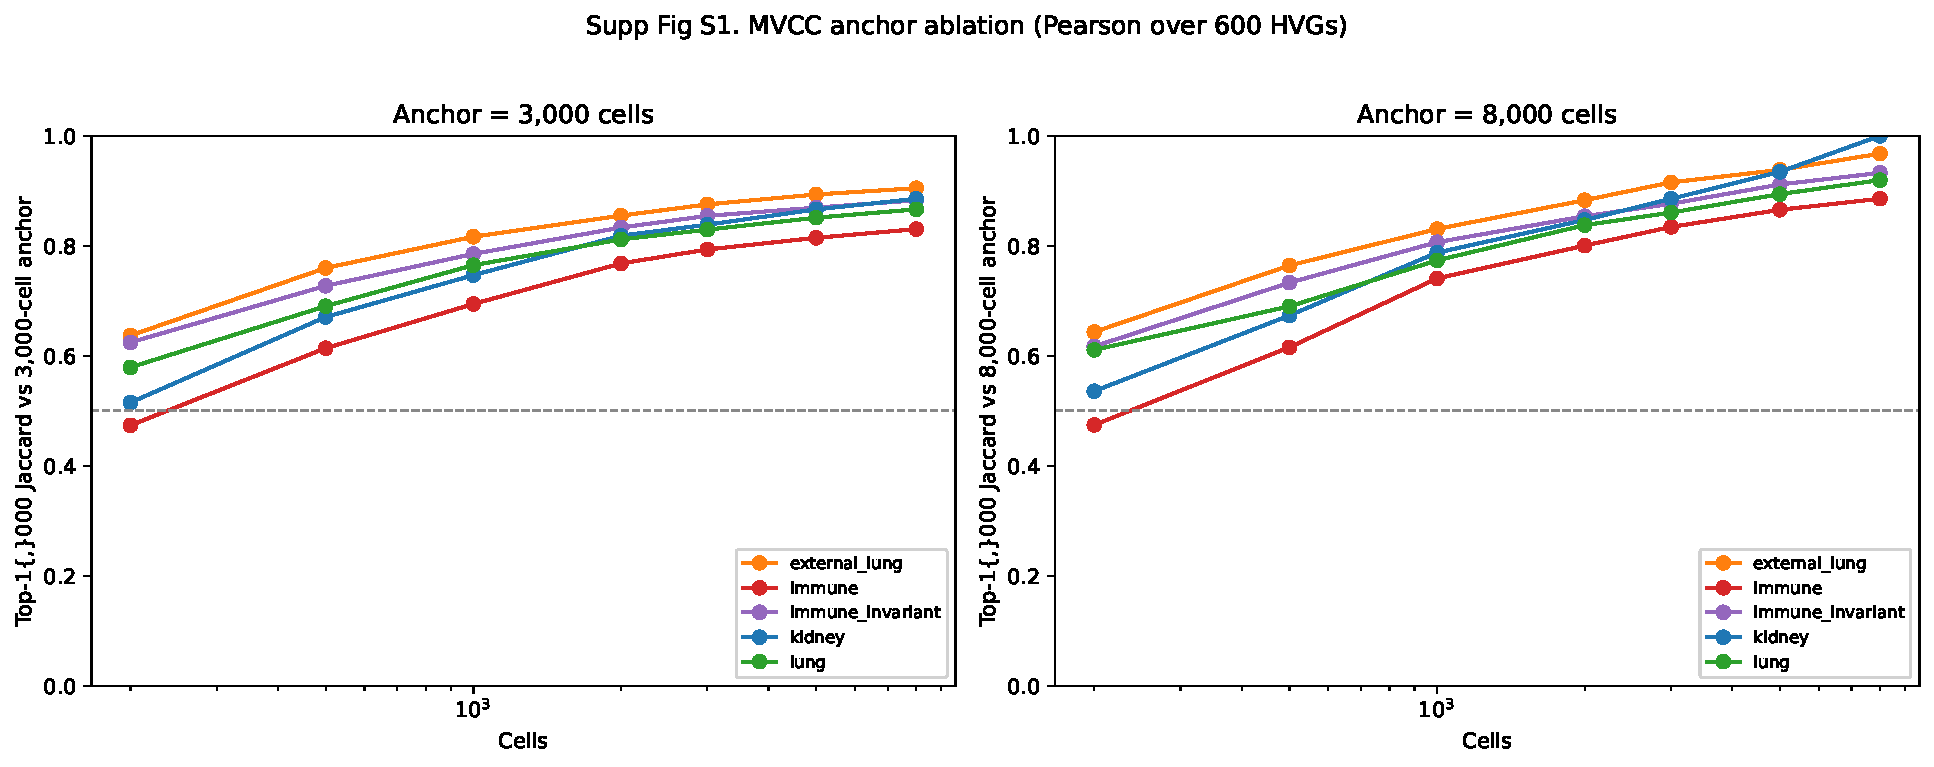
\includegraphics[width=\textwidth]{figures/supplementary/fig_s1_mvcc_anchor.pdf}
\caption{\textbf{MVCC anchor sensitivity.} Per-cohort, per-anchor
top-1{,}000 Jaccard against subsampled rankings under Pearson
correlation on 600 HVGs. Solid lines: 3{,}000-cell anchor; dashed
lines: 8{,}000-cell anchor (and 15{,}000-cell anchor for Delorey).
The MVCC values reported in Fig.\,1B of the main paper coincide
across anchors, demonstrating anchor-invariance.}
\label{fig:s1_mvcc}
\end{figure}

\begin{figure}[ht]
\centering
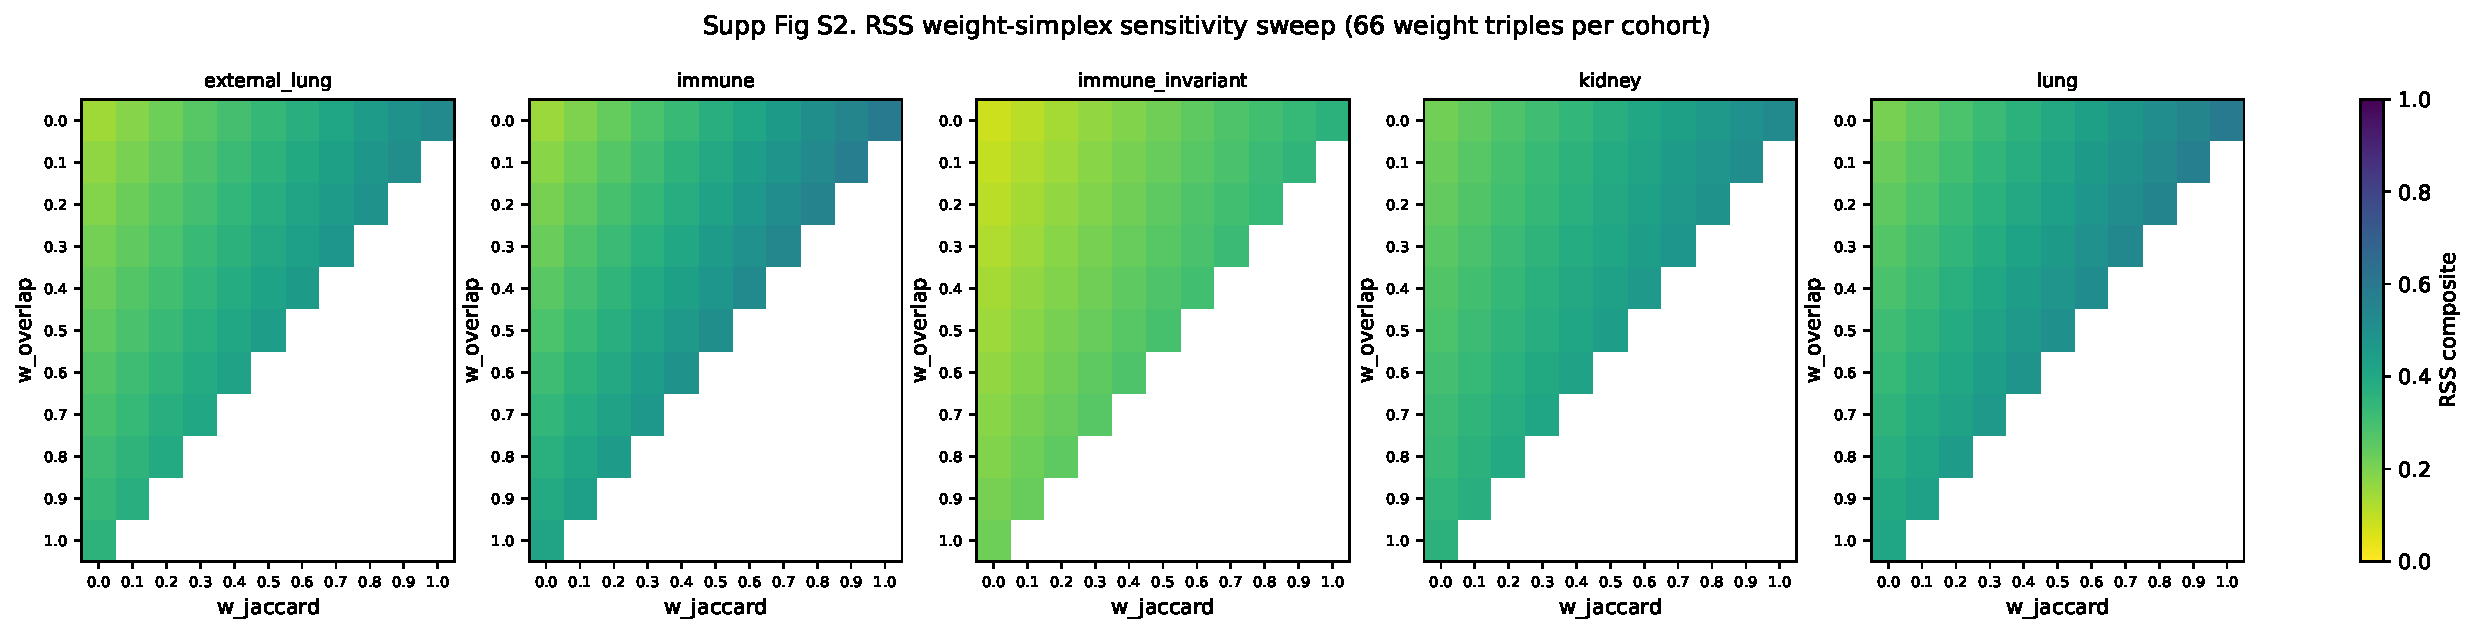
\includegraphics[width=\textwidth]{figures/supplementary/fig_s2_weight_simplex.pdf}
\caption{\textbf{RSS weight-simplex sensitivity.} Each panel shows the
recommendation produced at every point of the 66-point simplex
$(w_o, w_j, w_d)$ with each coordinate $\in \{0, 0.1, \ldots, 1.0\}$
and $w_o + w_j + w_d = 1$, evaluated on Axis 2 RSS. The dual-null
recommendation is invariant across the simplex because the
within-coarse null fails universally; the base-RSS recommendation
varies only at the boundary.}
\label{fig:s2_weight_simplex}
\end{figure}

\begin{figure}[ht]
\centering
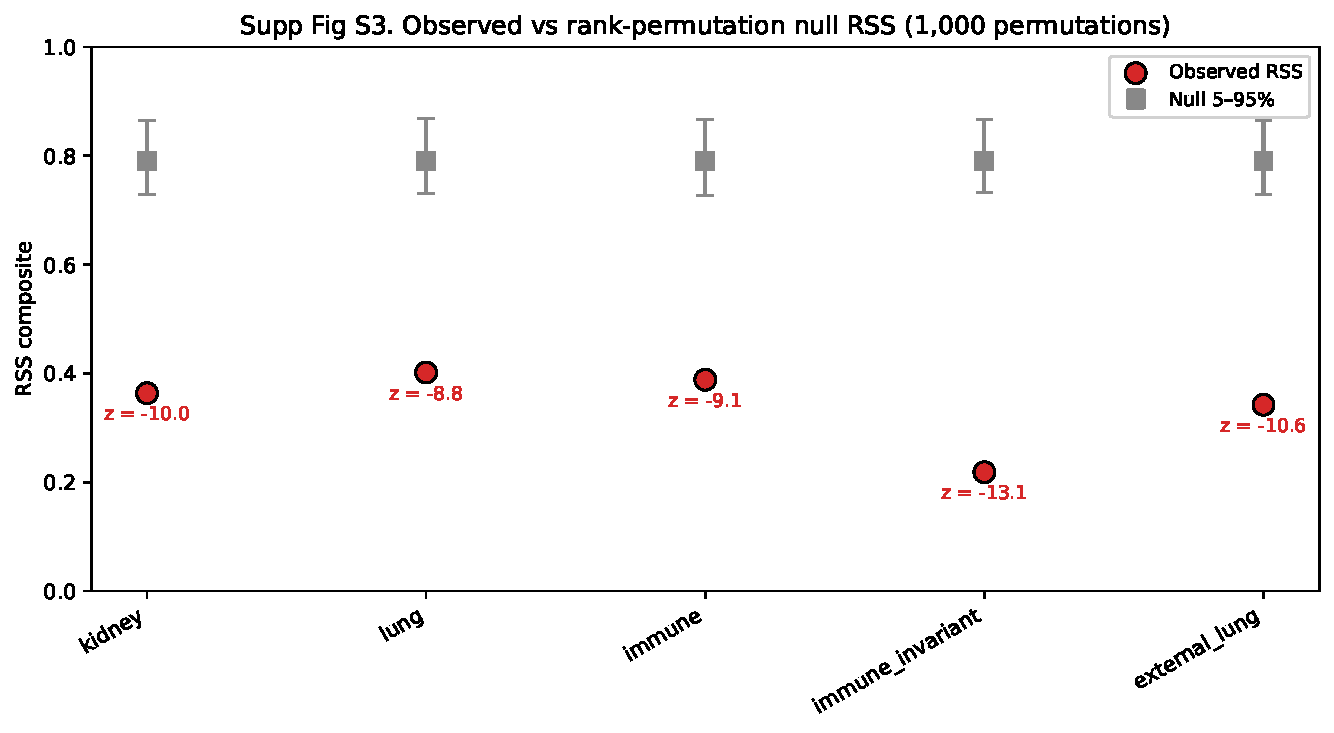
\includegraphics[width=\textwidth]{figures/supplementary/fig_s3_rss_null.pdf}
\caption{\textbf{Empirical null distribution of the bounded-drift RSS
under rank permutation.} Histograms show 1{,}000 permutation draws
per cohort; vertical line marks the observed RSS. Every observed
value sits 8.8 to 13.1 standard deviations below the null mean
($\approx 0.79$); empirical $p = 0.001$ (the floor) for every cohort.}
\label{fig:s3_rss_null}
\end{figure}

\begin{figure}[ht]
\centering
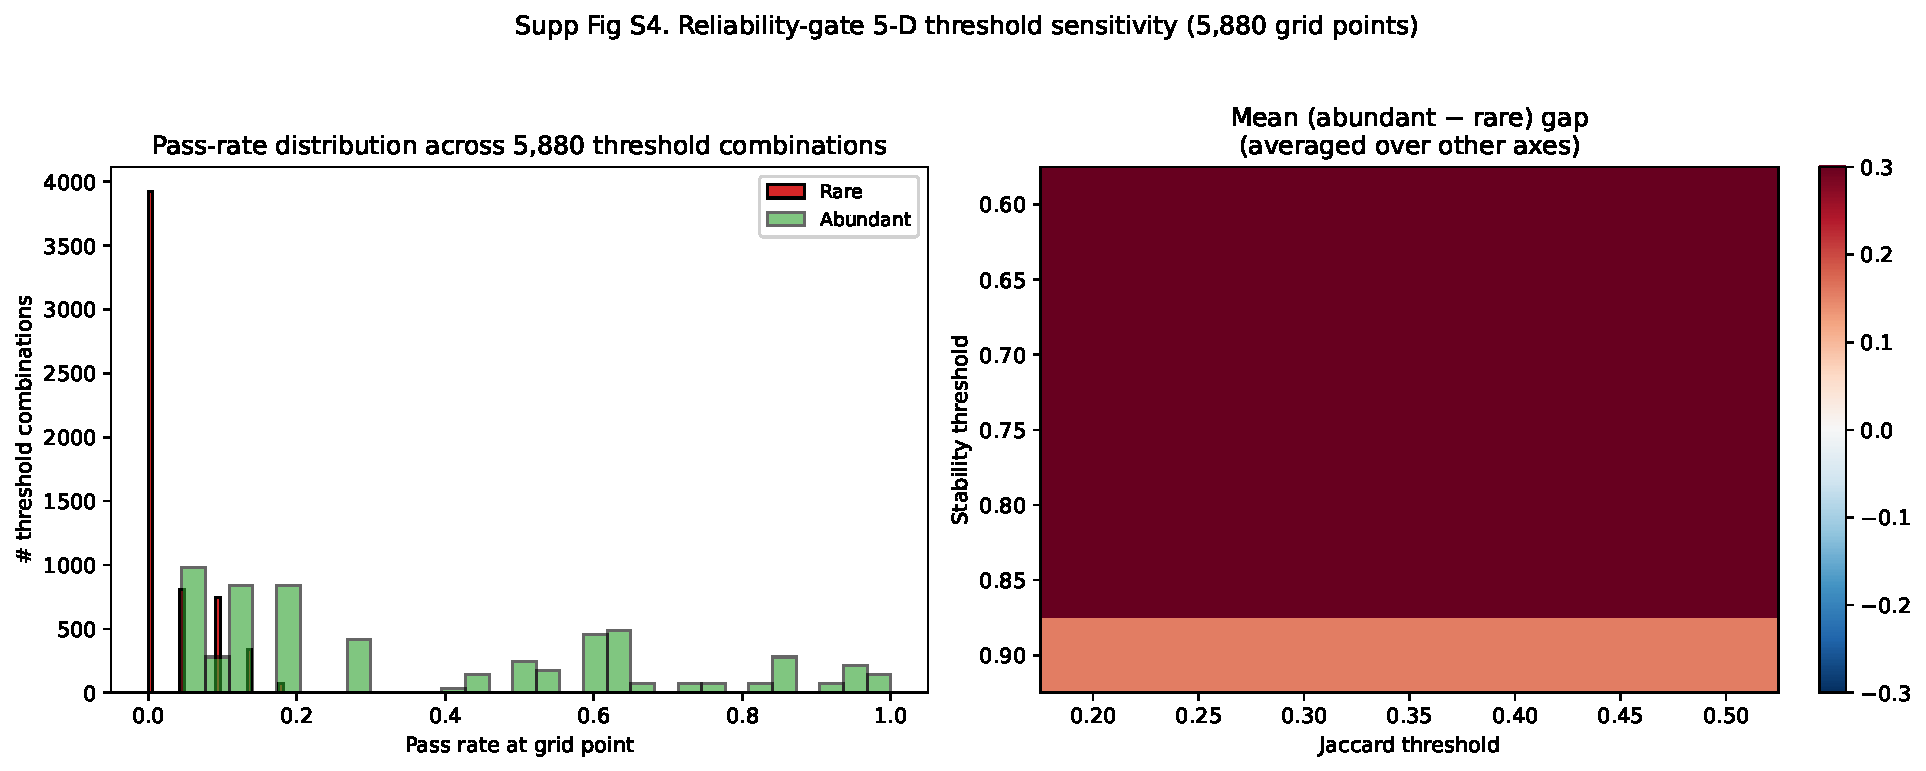
\includegraphics[width=\textwidth]{figures/supplementary/fig_s4_threshold_grid.pdf}
\caption{\textbf{Reliability-gate threshold-sensitivity heatmap.}
Pass-rate gap (abundant minus rare) over the 5{,}880-point
five-dimensional grid (stability, Jaccard, AUC, tail gap, cell
count). The gap direction is preserved at 100\% of grid points; the
primary-threshold gap (+0.182) is conservative relative to the grid
mean (+0.344).}
\label{fig:s4_threshold_grid}
\end{figure}

\begin{figure}[ht]
\centering
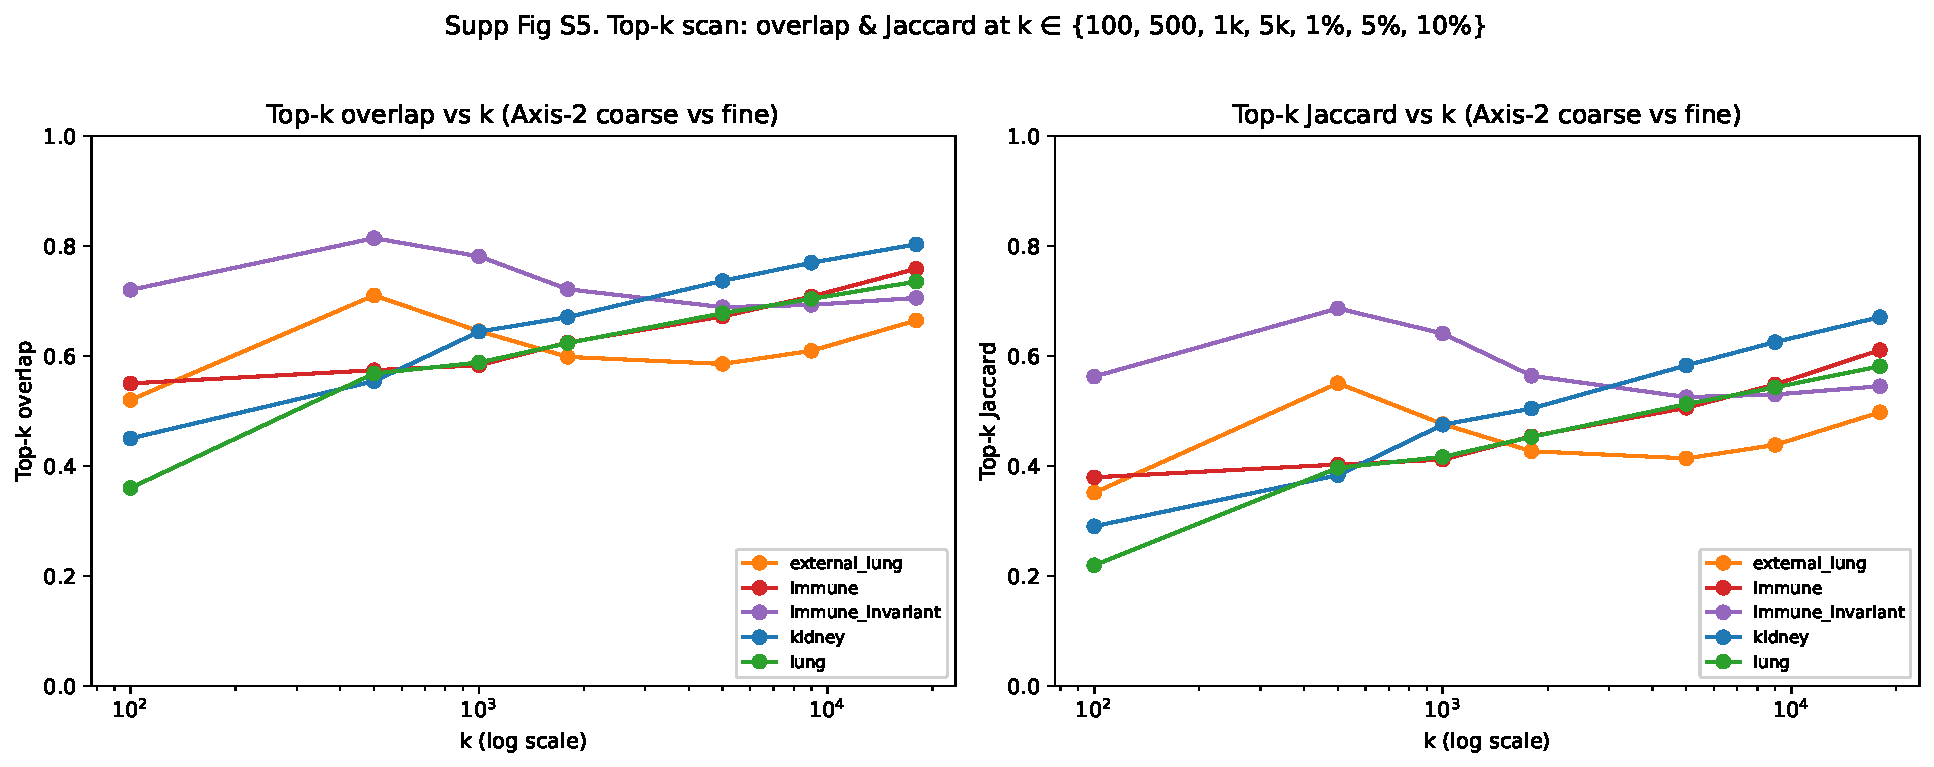
\includegraphics[width=\textwidth]{figures/supplementary/fig_s5_topk_scan.pdf}
\caption{\textbf{Top-$k$ scan and per-target overlaps.} Top-$k$
overlap and Jaccard at $k \in \{100, 500, 1{,}000, 5{,}000\}$ plus
top-1\%, top-5\%, and top-10\% of the edge universe, and per-target
top-5 and top-10 overlaps. Curves remain qualitatively consistent
across $k$, addressing the concern that the headline Jaccard at
$k=1{,}000$ might be artefactual to the chosen $k$.}
\label{fig:s5_topk_scan}
\end{figure}

\begin{figure}[ht]
\centering
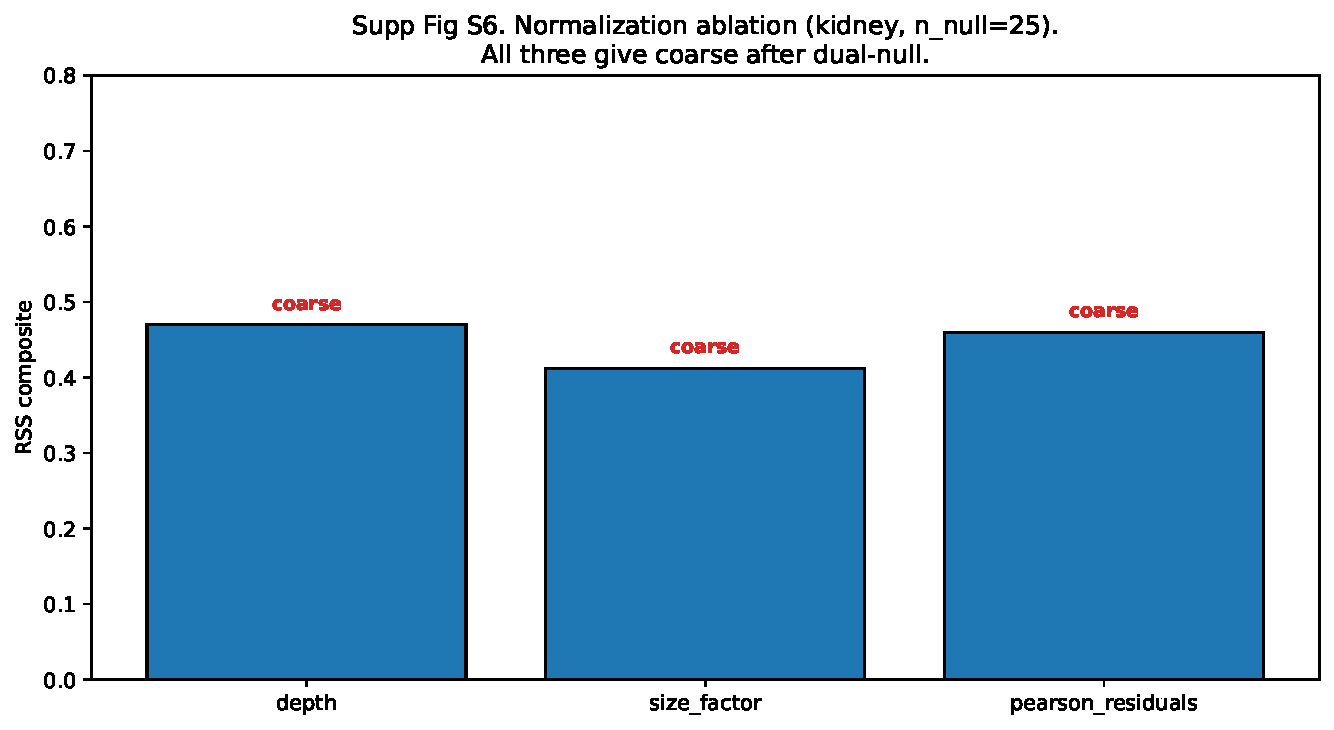
\includegraphics[width=\textwidth]{figures/supplementary/fig_s6_normalization.pdf}
\caption{\textbf{Normalization ablation on Axis 2 / kidney.} Three
schemes compared: depth + log1p (default), median-ratio size-factor +
log1p, and analytic Pearson residuals (Lause et al., 2021). All three
schemes produce the same calibrated recommendation (\emph{coarse}),
rebutting the concern that depth-normalization-induced variance
inflation drives the within-coarse failure.}
\label{fig:s6_normalization}
\end{figure}

\begin{figure}[ht]
\centering
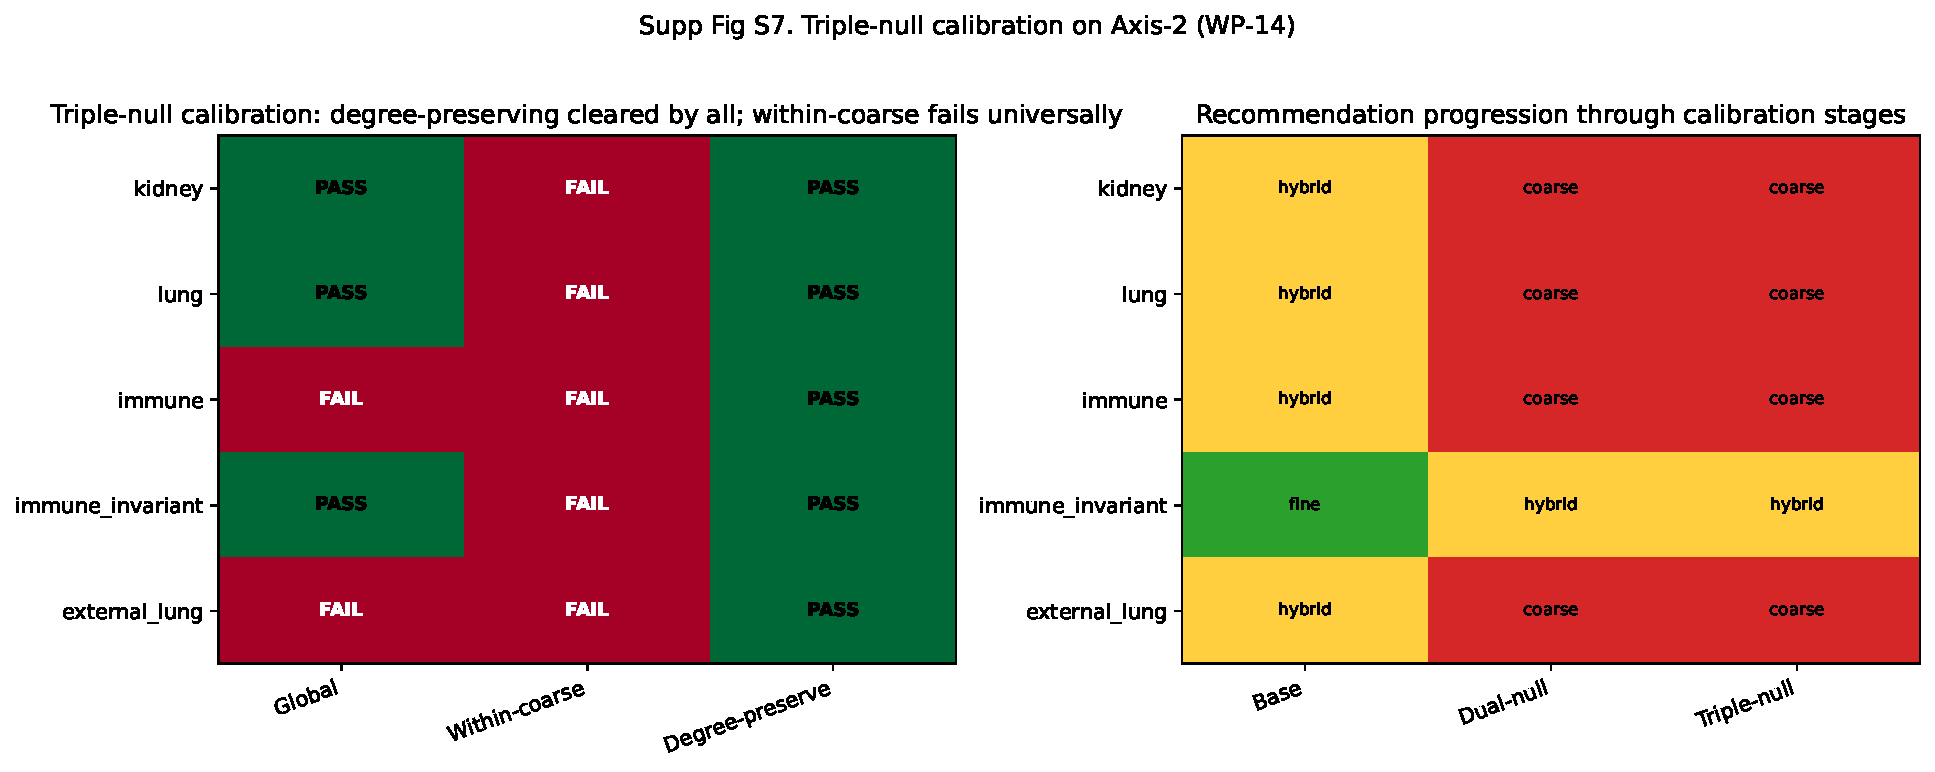
\includegraphics[width=\textwidth]{figures/supplementary/fig_s7_triple_null.pdf}
\caption{\textbf{Triple-null calibration.} A degree-preserving
bipartite edge-rewire null is added as a third, deliberately
permissive null family. Every cohort clears it at the permutation
floor ($p = 0.02$) while continuing to fail the within-coarse
constrained shuffle at $p \geq 0.22$, demonstrating that the
within-coarse failure reflects genuine over-partitioning of the
coarse cell types rather than null over-stringency.}
\label{fig:s7_triple_null}
\end{figure}

\end{document}
